\subsubsection{Venue}
	The venue selection module will be used by third-party UPRM users and will thus have minimum functionality available. The users should be able to create new venues, update the venues and delete venues. The user should also be able to view submissions and give feedback and mark the status of a project after review.\\ \\
	\textbf{Use Cases:}
	\begin{itemize}
		\item Creation of a venue.
		\item Updating of a venue.
		\item Deletion of a venue.
		\item Sending feedback and updating status to a project.\\
	\end{itemize}
	\textbf{Venue Use Case Overview Diagram:}\\
	\centerline{\fbox{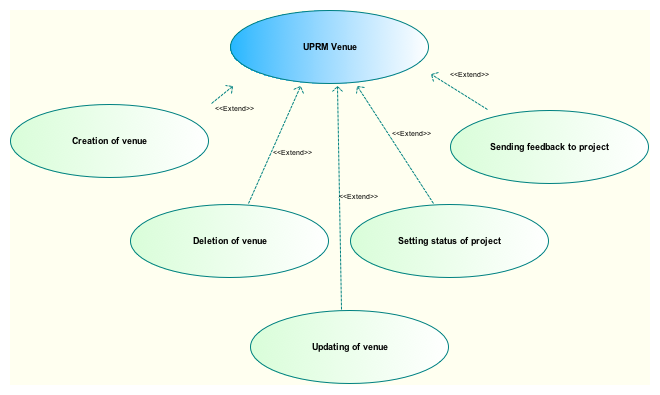
\includegraphics[scale=0.8]{venue/uprm_venueOverview.png}}}	